\chapter{Conclusiones}\label{ch:conclusiones}

Los objetivos de este proyecto estaban asociados
a la \textbf{creación de un sistema de componentes}
para el entorno de desarrollo \textit{JAMS}, que permita
a otros desarrolladores expandir las características
de la aplicación.

\textit{JAMS} es un entorno de desarrollo moderno,
flexible, modular y fácil de utilizar, donde el usuario
puede crear aplicaciones de una manera rápida y cómoda.
Las nuevas tecnologías desarrolladas en este
Trabajo Fin de Grado hacen posible \textbf{mantener esta arquitectura}
flexible y modular, permitiendo a otros desarrolladores
añadir funcionalidades sin tener que modificar el propio
código de la aplicación.

Para probar el funcionamiento de todas estas tecnologías
se ha desarrollado un componente que añade un \textbf{entorno
de desarrollo integrado} para el desarrollo de videojuegos
para la consola \textit{NES}.
Gracias a la creación de este componente, las tecnologías
utilizadas en \textit{JAMS} gozan de una arquitectura
flexible, pero robusta.

\section{Limitaciones}\label{sec:limitaciones}

Las tecnologías desarrolladas en este Trabajo
de Fin de Grado presentan las siguientes limitaciones:

\begin{itemize}
    \item \textbf{Velocidad}: el sistema de eventos
    presenta un rendimiento bastante bajo: su uso
    en el simulador \textbf{ralentiza la ejecución
    de manera considerable}.
    La búsqueda de gestores también tiende a ralentizar
    la ejecución de la aplicación.
    \item \textbf{Distribucción}: aunque crear componentes
    es un proceso sencillo, no existe ningun sistema de
    distribucción de componentes que los usuarios puedan
    utilizar, dejando este aspecto a cargo del desarrollador.
    Esta limitación puede resolverse creando una tienda de
    componentes donde los usuarios puedan descargar e instalar
    componentes fácilmente.
    \item \textbf{Falta de características}: el simulador
    incluido en el componente \textit{NES4JAMS} adolece
    de falta de herramientas: los usuarios no son
    capaces de añadir puntos de ruptura o visualizar
    las instrucciones ensambladas de su videojuego.
\end{itemize}

\begin{figure}[h]
    \centering
    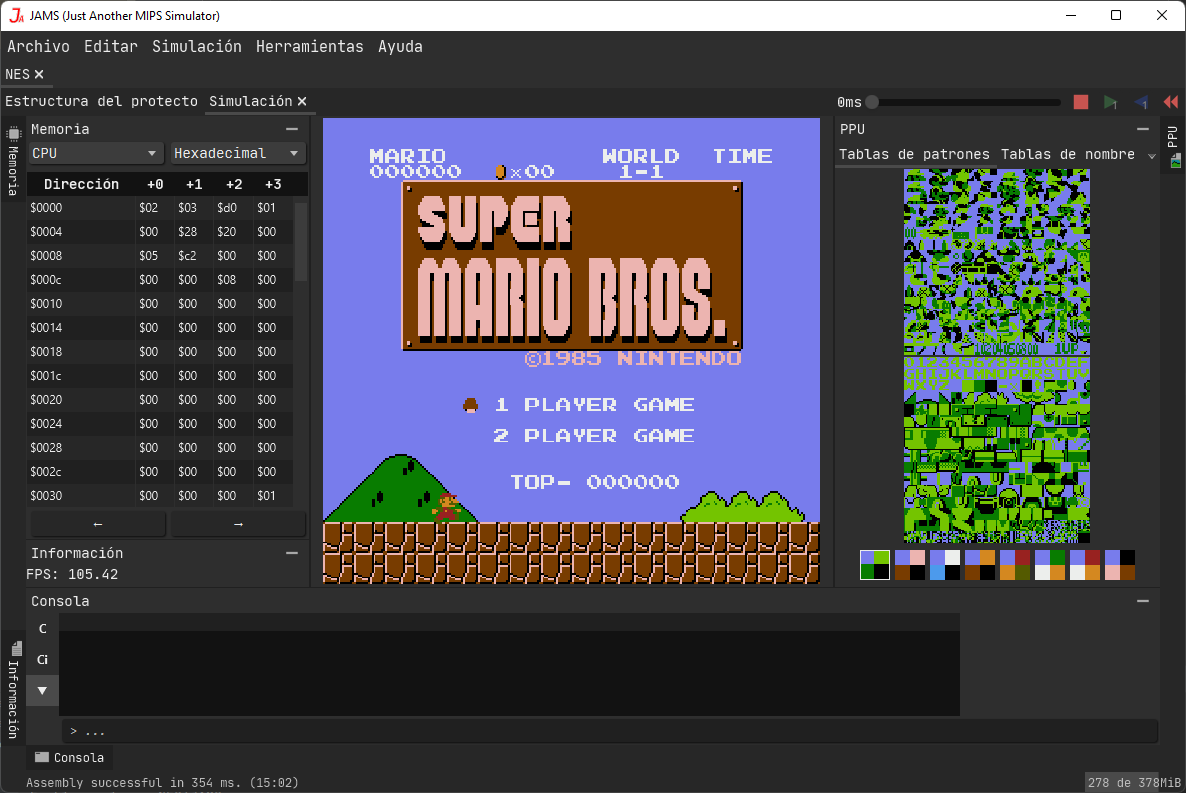
\includegraphics[width=0.8\textwidth]{images/conclusions/nes-simulator-tools}
    \caption{Todas las herramientas presentes en el simulador}
    \label{fig:nes-conclusions-tools}
\end{figure}

\section{Líneas futuras}\label{sec:líneas-futuras}

Tanto \textit{JAMS} como el componente \textit{NES4JAMS}
contarán con varias actualizaciones importantes en
el futuro cercano.

\begin{itemize}
    \item \textbf{Nuevas herramientas para el simulador}:
    como ya se ha mencionado, el simulador presente en
    \textit{NES4JAMS} carece de ciertas herramientas.
    La primera actualización para el componente añadirá
    algunas nuevas, como pueden ser un visualizador
    de instrucciones y la adición de puntos de ruptura.
    \item \textbf{Uso del \textit{Proyecto Valhalla}:} el
    \textit{Proyecto Valhalla}\cite{PROJECT_VALHALLA}, creado en 2014,
    está desarrollando una de las características más esperadas
    por los desarrolladores \textit{JAVA}: \textbf{paso por valor}.
    Esta característica permitirá optimizar de manera considerable
    todas las herramientas creadas en este Trabajo Fin
    de Grado.
    Estas nuevas características empezarán su desarrollo cuando esta
    tecnología esté en fase \textit{preview}.
\end{itemize}

\section{Reflexiones finales}\label{sec:reflexiones-finales}

El desarrollo de \textit{NES4JAMS}, junto con el
de \textit{JAMS}, ha supuesto el proyecto más complejo en el
que he trabajado:
este proyecto abarca un montón de conceptos y tecnologías
que deben sincronizarse perfectamente para que el resultado
sea robusto.
El desarrollo del sistema de componentes ha supuesto en una
vuelta al pasado, a tiempos en los que trabajé
en diferentes expansiones de videojuegos.

\textit{NES4JAMS} me ha permitido investigar el funcionamiento
de una de las consolas más importantes en la
historia del videojuego.
La capacidad de poder ejecutar videojuegos en una aplicación
desarrollada desde cero ha sido una experiencia muy gratificante.

Finalmente, agradecer a todas las personas que me han
estado apoyando en este proyecto, a mi familia, amigos y a mis
tutores Óscar y Luis, ya que gracias a ellos este trabajo
ha sido posible.
